\subsection{External Interfaces}
\label{requirements:interfaces}

%TODO: Description, copy from example

\subsubsection{User Interface} %Jan
\label{requirements:interfaces:user}
        
As described in section ?, this is how the final result could look like. Figure \ref{gui} is only a draft, trying to visualize how the integration into Tomboy can be accomplished.
\begin{figure}[h]
  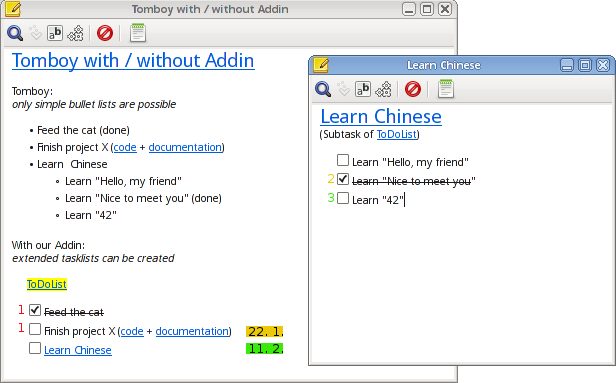
\includegraphics[width=\textwidth]{graphics/Screenshot_cropped_edited.png}
  \caption{GUI mockup}
  \label{gui}
\end{figure}

You can see the checkboxes for each of the todo items, along with some sample priorities to the left and some due dates to the right.

\begin{requirement}{Create TaskList}
  \desc{The user shall be able to create a new TaskList with a button or a shortcut text, like ``[]''. These lists expand automatically and contain individual Tasks that can be checked out when done.}
  \priority{1}
  \riskref{C}
\end{requirement}

\begin{requirement}{Edit TaskList}
  \desc{The user can easily add, remove and change single TaskList items, without using any complicated structures like menus etc.}
  \priority{1}
  \riskref{C}
\end{requirement}

\begin{requirement}{Priority}
  \desc{The user can (but does not have to) add and change priorities to individual Tasks and TaskLists.}
  \priority{1}
  \riskref{H}
\end{requirement}

\begin{requirement}{Due date}
  \desc{The user can (but does not have to) add and change due dates to individual Tasks and TaskLists, indicating when these should be finished. The system shows somehow graphically (for example with colors) when items are near or even over their due date.}
  \priority{1}
  \riskref{H}
\end{requirement}

\begin{requirement}{Create Subtasks}
  \desc{The user can (but does not have to) add Subtasks to individual Tasks. These Subtasks are in principal notes, but can themselves contain Tasks and TaskLists.}
  \priority{1}
  \riskref{H}
\end{requirement}

\begin{requirement}{Show / hide completed Tasks}
  \desc{The user has various possibilities to handle completed Tasks. He can show them crossed out, he can hide them, and he can possibly show them after the completed Tasks. }
  \priority{2}
  \riskref{M}
\end{requirement}

\begin{requirement}{Reorder TaskLists}
  \desc{The user has the possibility to order the TaskLists according to various criteria, like due date, priority, date added etc.}
  \priority{2}
  \riskref{L}
\end{requirement}

%	\subsubsection{Hardware Interfaces}
%	\label{requirements:interfaces:hardware}
	
	\subsubsection{Software Interfaces}
	\label{requirements:interfaces:software}
        %TODO => export (xml, evolution, tasque, ...)
        %     => Tomboy (save, ...)

	%\subsubsection{Communication Interfaces}
	%\label{requirements:interfaces:communication}
	

\subsection{Licensing Requirements}
\label{requirements:license}
%TODO: ...

\subsection{Supported Operating Systems}
\label{requirements:os}
%TODO: ...

\subsection{Language}
\label{requirements:language}
%TODO: ...

%TODO: Configuration

\subsection{Functional Requirements} % Gerd
\label{requirements:functional}
%TODO: export, import, all note browser stuff, show progress of subtasks (low priority/critically), taskgraph(image),

\begin{requirement}{Interface Requirement}
  \desc{insert description}
  \priority{1}
  \riskref{C}
\end{requirement}


%\subsection{Performance Requirements}
%\label{requirements:performance}

\subsection{Design Constraints}
\label{requirements:constraints}
% => modules (textbuffer, note gui, notes window gui)

\subsection{Quality Requirements}
\label{requirements:quality}
% => Bugs, unit tests

%\subsection{Other Requirements}
%\label{requirements:other}
